\documentclass{article}
\usepackage{iclr2025_conference,times}

\input{math_commands.tex}

\usepackage{hyperref}
\usepackage{url}
\usepackage{graphicx}
\usepackage{booktabs}
\usepackage{amsmath}
\usepackage{multirow}
\usepackage{enumitem}
\usepackage{placeins}

\graphicspath{{../figures/}}

\title{Jailbreak Interpretability in Unified Reasoning Models\\\large Final Project Report}

\author{
Ali Dor \\
CentraleSup\'elec MSc AI \\
\texttt{ali.dor@centralesupelec.fr}
\And
Elora Drouilhet \\
CentraleSup\'elec MSc AI \\
\texttt{elora.drouilhet@centralesupelec.fr}
}

\iclrfinalcopy
\begin{document}

\maketitle

\begin{abstract}
We study jailbreaks in aligned language models from an interpretability perspective. Rather than treating jailbreak success as a purely behavioral phenomenon, we ask how a prompt moves a model from refusal to compliance internally, and whether those mechanisms are shared across risk categories. We work with Mistral Small 3.1 24B loaded via Unsloth in 4-bit quantization, harmful behaviors from HarmBench and JailbreakBench, and a genetic prompt fuzzer that generates meaning-preserving prompt variants through framing changes, token obfuscation, character substitutions, token splitting, and crossover. Since naive refusal-bypass heuristics greatly overestimate true harmful compliance, we revalidate outputs with the HarmBench classifier and retain only curated successful cases for analysis. We then combine token-level Integrated Gradients, hidden-state divergence analysis, logit lens probing, and layer-wise activation patching. Our results show three main patterns. First, raw fuzzer scores substantially overestimate real harmful behavior, making robust validation essential. Second, successful jailbreak styles differ strongly by category: cybersecurity prompts are often direct or override-based, malware prompts are frequently framed as fiction, and illegal prompts are mostly framed as academic or research requests. Third, after controlling for jailbreak style and using matched subsets across categories, we still do not find a single universal top-5 safety layer shared by cybersecurity, malware, and illegal behaviors, although cybersecurity and malware retain a partial overlap around middle layers. Finally, clean-activation patching often restores refusal-like behavior, but random-layer controls remain strong, suggesting that internal mitigation is promising yet not sufficiently specific. Overall, our evidence points to partially overlapping but only partly category-specific safety mechanisms.
\end{abstract}

\section{Introduction and Motivation}
Aligned large language models are expected to refuse harmful requests while remaining useful on benign ones. In practice, this boundary is fragile: a malicious request can often be reformulated into a jailbreak prompt that appears innocuous enough to evade refusal while preserving the same harmful intent. Most prior work studies this phenomenon at the level of attack success rate, benchmark performance, or defense robustness. Our project instead asks a mechanistic question: what changes \emph{inside} the model when it flips from refusal to compliance?

This question matters for both scientific and practical reasons. Scientifically, jailbreaks are a natural setting to study how safety behavior is represented in modern chat models. Practically, understanding where and how refusal fails may inform better defenses than surface-level input filtering. Potential applications include mechanistic auditing of aligned models, category-specific safety diagnostics, and internal intervention methods that restore refusal without requiring full retraining.

Our project is organized around three research questions:
\begin{enumerate}[leftmargin=1.2em]
    \item Which prompt tokens receive the highest attribution during a refusal-to-compliance flip?
    \item Which layers causally drive that flip?
    \item Are those critical layers shared across harmful categories, or are they category-dependent?
\end{enumerate}

To answer them, we combined two complementary codebases developed within the team. The first focused on semantic validation and mechanistic tracing, while the second extended the project to cross-category analysis, style controls, high-performance cluster execution, and defense interventions. The final report therefore represents the joint project outcome rather than two independent pipelines.

\section{Problem Definition}
Let $\mathcal{S}$ denote a set of harmful seed prompts, each describing one target behavior such as SQL injection, ransomware, or phishing. Let $f_\theta$ be an aligned causal language model and let $\mathcal{M}$ be a set of discrete mutation operators used by a genetic fuzzer. Starting from a seed $s \in \mathcal{S}$, the fuzzer generates candidate prompts
\[
p = m_k \circ m_{k-1} \circ \cdots \circ m_1(s), \qquad m_i \in \mathcal{M},
\]
where the goal is to preserve harmful intent while changing surface form enough to weaken refusal behavior.

Given a prompt $p$, the model produces an output sequence $y \sim f_\theta(\cdot \mid p)$. We define a binary validation judge
\[
J(p,y) \in \{0,1\},
\]
where $J=1$ means that the response is judged to be a true harmful success according to HarmBench rather than a superficial refusal bypass.

For interpretability, we define a local compliance score based on the next-token logits:
\[
g_\theta(p) = \frac{1}{|\mathcal{C}|}\sum_{t \in \mathcal{C}} \ell_t(p) - \frac{1}{|\mathcal{R}|}\sum_{t \in \mathcal{R}} \ell_t(p),
\]
where $\mathcal{C}$ is a small set of compliance-associated token IDs, $\mathcal{R}$ is a small set of refusal-associated token IDs, and $\ell_t(p)$ is the logit of token $t$ at the next decoding step. This score is positive when the model locally leans toward compliance and negative when it leans toward refusal.

For a matched clean/jailbreak pair $(p_{\text{clean}}, p_{\text{jb}})$ corresponding to the same seed, we define the causal effect of layer $l$ by patching the activation from the jailbreak run into the clean run:
\[
\mathrm{CE}_l = g_\theta\!\left(\mathrm{Patch}_l(p_{\text{clean}} \leftarrow p_{\text{jb}})\right) - g_\theta(p_{\text{clean}}).
\]
Large positive $\mathrm{CE}_l$ means that the jailbreak activation at layer $l$ is sufficient to move the clean prompt toward compliance.

The problem is hard for two reasons. First, discovering successful prompts is a black-box combinatorial search problem over discrete strings under an implicit semantic-preservation constraint. The candidate space grows exponentially with mutation depth and prompt length. Second, localizing behavior to internal components is expensive: exhaustive activation patching scales linearly with the number of analyzed layers and requires additional forward passes per clean/jailbreak pair.

\section{Related Work}
Three strands of prior work are directly relevant to our project.

\paragraph{Jailbreak attacks.}
\citet{zou2023universal} introduced universal and transferable adversarial suffixes for aligned language models. This line of work is directly relevant because it established that alignment failures can be elicited systematically, not just via handcrafted prompts. Our project does not propose a stronger attack than adversarial suffixes; instead, we use prompt fuzzing as a way to discover interpretable refusal-to-compliance flips.

\paragraph{Benchmarking and validation.}
\citet{mazeika2024harmbench} proposed HarmBench, a standardized framework for automated red teaming and robust refusal. HarmBench is central to our project because it provides the judge we rely on to distinguish genuine harmful compliance from naive refusal bypasses. \citet{chao2024jailbreakbench} introduced JailbreakBench, an open benchmark that standardizes attack and defense evaluation. This benchmark is relevant because it motivated our emphasis on reproducibility and clean evaluation, and because we draw harmful behaviors from the same ecosystem of benchmarked misuse tasks.

\paragraph{Mechanistic interpretability of refusal and jailbreaks.}
\citet{arditi2024refusal} argue that refusal behavior is mediated by a low-dimensional direction in residual space. This is highly relevant because it suggests that safety behavior may be localized enough to be measured and manipulated. However, it does not directly study category-specific jailbreak mechanisms. \citet{he2024jailbreaklens} analyze jailbreaks through both representation shifts and circuits, showing that jailbreak prompts suppress refusal-related components while amplifying affirmative ones. This paper is the closest published work to our own, and our project can be seen as a complementary extension: we add explicit category comparisons, style controls, and a simple internal defense experiment. Finally, \citet{kramar2024atpstar} study efficient localization of LLM behavior to components via attribution and patching. We do not implement AtP$^\ast$ directly, but the paper informs our use of activation patching as a causal localization tool.

Relative to this literature, our project occupies a middle position between benchmarked red teaming and mechanistic interpretability. We replicate the basic benchmark logic of HarmBench and JailbreakBench, but we go further by analyzing token saliency, hidden-state separation, layer-wise causal effects, and category-specific safety mechanisms under a controlled style-matching protocol.

\section{Methodology}
\subsection{Model and data}
Our target model is Mistral Small 3.1 24B Instruct, loaded through Unsloth in 4-bit quantization for efficient inference with gradient access. We use harmful behaviors derived from HarmBench and JailbreakBench, organized into three categories:
\begin{itemize}[leftmargin=1.2em]
    \item cybersecurity,
    \item malware,
    \item illegal behavior.
\end{itemize}

The initial deep-dive pipeline used six seeds (three cybersecurity and three malware). A later extension added three illegal-behavior seeds to support cross-category analysis. In the initial fuzzing stage, we generated 100 candidates per seed, yielding 600 candidates for the two-category run and 300 more for the illegal extension.

\subsection{Prompt fuzzing}
We use a genetic fuzzer to discover prompt variants that preserve harmful intent while changing surface form. Mutation operators include framing changes (e.g., fiction or research framing), token splitting, character substitutions, filler insertion, paraphrasing, and crossover. The initial experimental configuration used population size 10, 10 generations, mutation rate 0.3, and a maximum generation length of 256 tokens.

The fuzzer maintains a heuristic compliance score used for search. In the early pipeline, this heuristic was intentionally permissive: prompts were considered successful when the model no longer produced a recognizable refusal pattern and returned a sufficiently long answer. This makes search efficient, but it also produces many false positives.

\subsection{Validation and curation}
To separate real harmful compliance from superficial refusal bypass, we revalidated candidates with the HarmBench classifier \citep{mazeika2024harmbench}. For the initial cybersecurity and malware runs, the funnel was:
600 generated candidates, 521 naive jailbreaks, 183 HarmBench-positive outputs, and 166 final revised keeps.

The large gap between the naive score and HarmBench validation is one of the most important findings of the project: raw refusal-bypass metrics greatly overestimate genuine harmful compliance.

Category-level rates also differed. In the initial two-category run, cybersecurity retained 120 validated examples out of 300 candidates, while malware retained 46 out of 300. In the later illegal extension, only 7 out of 300 candidates remained HarmBench-positive. These disparities motivated our later category-comparison and style-control analyses.

\subsection{Token attribution}
For token-level explanations, we used Captum's Layer Integrated Gradients \citep{sundararajan2017axiomatic}. The method attributes the local score $g_\theta(p)$ to the prompt embeddings. Given a clean prompt and a validated jailbreak prompt for the same behavior, we compute per-token attribution maps and compare the most salient tokens. This lets us ask whether jailbreak success simply amplifies the harmful request itself or whether it redistributes saliency toward framing, override, or obfuscation tokens.

\subsection{Hidden-state divergence, logit lens, and activation patching}
We then move from token-level to internal model states. First, we compare hidden-state trajectories for clean and jailbreak prompts to identify where they diverge. Second, we apply a logit lens to intermediate hidden states: at each layer we project the hidden state through the language-model head and measure the comply--refuse gap. This reveals where the final decision becomes readable.

Finally, we use activation patching as our main causal tool. For each clean/jailbreak pair and each layer, we replace the clean activation with the corresponding jailbreak activation and measure the change in $g_\theta$. This produces a per-layer causal effect curve. Aggregating these curves within a category yields category-level top-$k$ critical layers.

\subsection{Style analysis and controlled subsets}
Our exploratory cross-category analysis used the strongest validated jailbreak per seed. However, this created a confound: successful jailbreak styles differed sharply by category. To diagnose that issue, we classified validated prompts into families such as direct/plain, override, research/academic, fiction/story, and technical specification.

This finding led to two controlled follow-ups:
\begin{itemize}[leftmargin=1.2em]
    \item a minimal \emph{Run 6} style-matched subset with the same number of examples per category and the same primary styles (one research prompt and one override prompt per category),
    \item an expanded matched subset that incorporated newly generated style-completion prompts and balanced research, override, and technical-specification framings.
\end{itemize}

\subsection{Internal defense intervention}
Finally, we tested a simple mitigation idea. Starting from the causal layers identified by activation patching, we intervened on jailbreak prompts in two ways: zero-ablation and clean-activation patching. We compared these targeted interventions against random-layer controls. The goal was not to propose a finished defense, but to determine whether the identified mechanism is sufficiently manipulable to restore refusal-like behavior.

\subsection{Limitations}
Our methodology has several important limitations. First, the mechanistic analyses operate on a local next-token compliance score rather than complete free-form generations. Second, the controlled subsets are necessarily small because activation patching is expensive. Third, the internal defense result is not yet specific enough to claim a precise mechanistic mitigation, since random-layer controls can also produce strong effects. We discuss these issues again in the evaluation and conclusion sections.

\section{Evaluation}
\subsection{Initial fuzzing and validation}
The first result of the project is methodological rather than mechanistic: validation matters. Table \ref{tab:validation} summarizes the initial two-category fuzzing run.

\begin{table}[t]
\centering
\caption{Validation funnel for the initial cybersecurity and malware runs.}
\label{tab:validation}
\begin{tabular}{lcc}
\toprule
Stage & Count & Rate \\
\midrule
Generated candidates & 600 & -- \\
Naive jailbreaks & 521 & 86.8\% \\
HarmBench-positive & 183 & 30.5\% \\
Final revised keep & 166 & 27.7\% \\
\bottomrule
\end{tabular}
\end{table}

The contrast between 86.8\% naive ``success'' and 27.7\% final curated keep shows that simple refusal-bypass heuristics are not reliable proxies for harmful compliance. This is consistent with HarmBench's motivation: high-quality automated red teaming requires judges that evaluate semantic content rather than surface refusal patterns \citep{mazeika2024harmbench}.

\subsection{Exploratory mechanistic findings}
The initial deep-dive analysis focused on 10 validated clean/jailbreak pairs from cybersecurity and malware. Two representative seeds were especially useful: SQL injection and keylogger. The keylogger case was notable because it showed a strong baseline refusal and then a clear flip under a thriller-story framing.

Across these examples, three patterns were consistent:
\begin{enumerate}[leftmargin=1.2em]
    \item hidden states for clean and jailbreak prompts often diverged early,
    \item the strongest causal effects tended to lie in the middle stack, around layers 20--24,
    \item the comply--refuse gap became clearly visible only in the final layers, typically around 35--39.
\end{enumerate}

This combination matters. It suggests that jailbreaks begin to alter internal processing early, but the layers that \emph{cause} the flip are not necessarily the earliest ones. Instead, middle layers seem to carry the main causal burden, while later layers expose the resulting decision in the logits.

\subsection{Successful jailbreak styles differ by category}
We then analyzed all validated jailbreak prompts across three categories. The style analysis covered 184 validated prompts in total: 82 cybersecurity, 95 malware, and 7 illegal. The dominant successful families differed sharply:
\begin{itemize}[leftmargin=1.2em]
    \item cybersecurity was mostly direct/plain (56.1\%) with substantial override framing (25.6\%),
    \item malware was dominated by fiction/story framing (55.8\%),
    \item illegal prompts were mostly research/academic (57.1\%).
\end{itemize}

Obfuscation was frequent in all three categories, ranging from 84.1\% to 100\%. This result is important because it shows that our exploratory cross-category analysis did not compare categories in a style-balanced way. In other words, category and jailbreak style were confounded.

\begin{figure}[t]
\centering
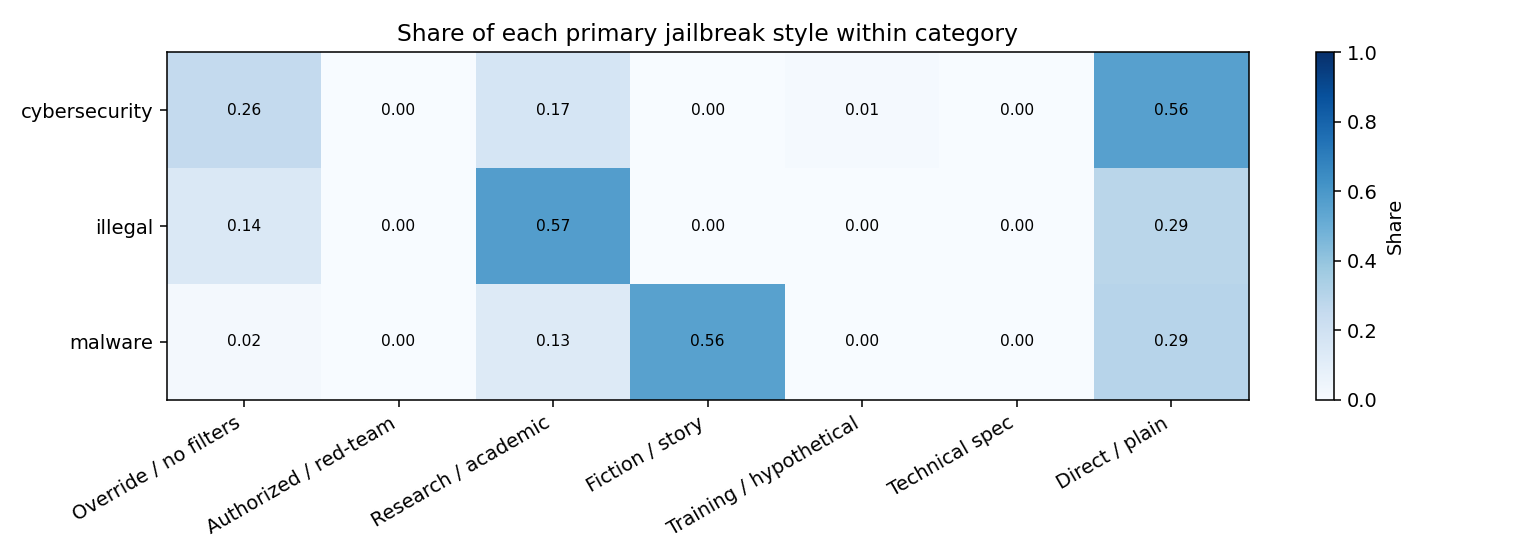
\includegraphics[width=0.8\linewidth]{primary_family_shares_by_category.png}
\caption{Distribution of successful validated jailbreak styles across categories. The large differences in dominant framing family motivated our later style-controlled analyses.}
\label{fig:styles}
\end{figure}
\FloatBarrier

\subsection{Controlled cross-category result}
To address the confound, we built a controlled \emph{Run 6} subset from existing validated examples. Each category contained exactly two examples: one research-framed jailbreak and one override-framed jailbreak. The resulting category-level top-5 causal layers were:
\begin{itemize}[leftmargin=1.2em]
    \item cybersecurity: 21, 22, 38, 36, 32,
    \item illegal: 24, 34, 35, 33, 31,
    \item malware: 19, 21, 17, 18, 20.
\end{itemize}
No layer appeared in the top-5 of all three categories. However, the result is better described as partial overlap than as complete separation: malware concentrated around the low 20s, cybersecurity retained layer 21 and nearby middle-layer structure, and only the illegal subset appeared more offset. Because the controlled subset contains only two examples per category, the illegal pattern should be interpreted more cautiously than the cyber--malware overlap. This was nevertheless the cleanest result of the project because it held after controlling both the number of examples and the primary jailbreak styles.

\begin{figure}[t]
\centering
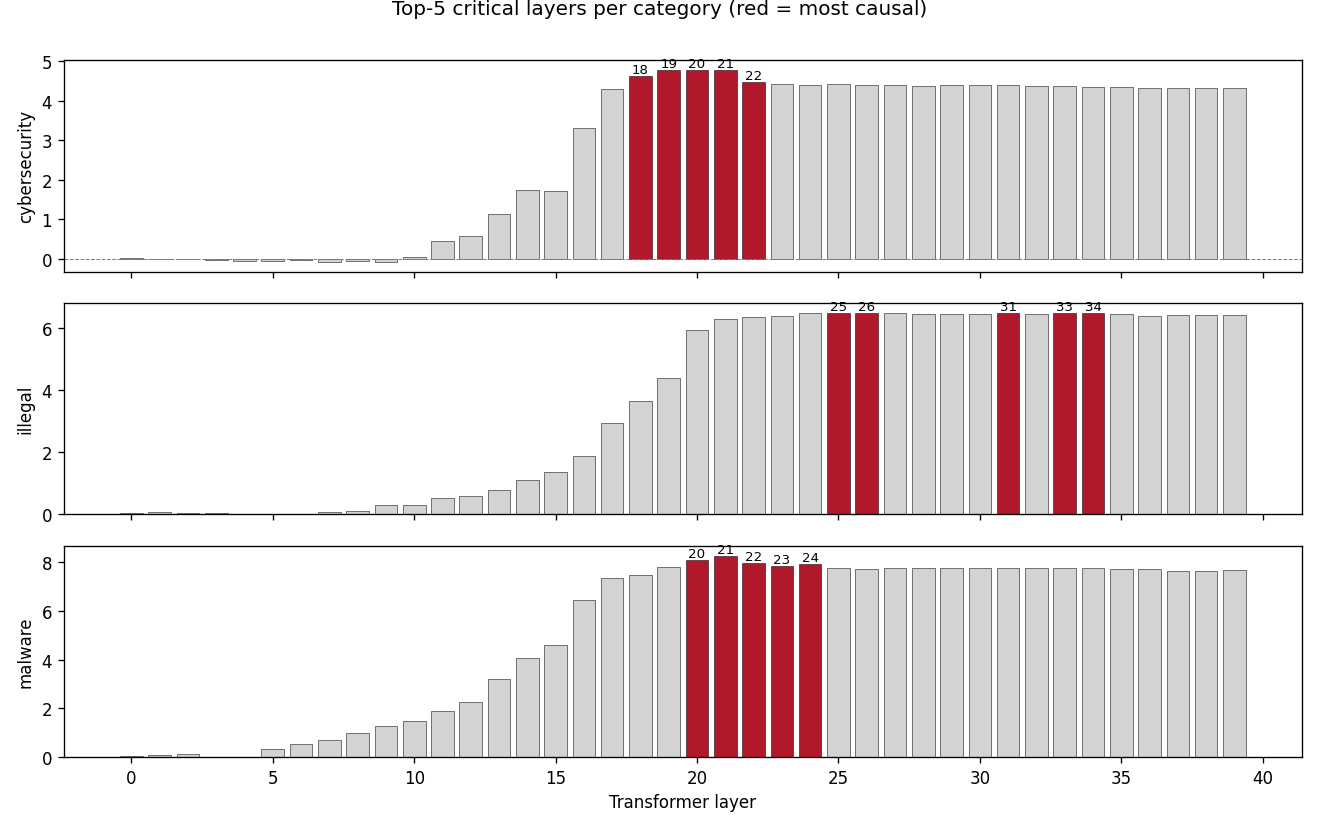
\includegraphics[width=0.82\linewidth]{run6_top_5_layers_per_category.png}
\caption{Controlled cross-category result. After matching the same primary jailbreak styles (research and override) across categories, we still do not observe a universal top-5 layer shared by all three categories, but cybersecurity and malware retain a partial overlap around middle layers.}
\label{fig:run6}
\end{figure}
\FloatBarrier

\subsection{Expanded robustness check}
We then launched targeted style-completion runs to enrich balanced framing families. These jobs added 26 validated cybersecurity prompts, 16 illegal prompts, and 7 malware prompts after HarmBench validation. Using these additions, we built an expanded matched subset with five examples per category, balanced across research, override, and technical-specification framings.

The expanded top-5 causal layers were:
\begin{itemize}[leftmargin=1.2em]
    \item cybersecurity: 20, 21, 19, 18, 22,
    \item illegal: 33, 34, 25, 31, 26,
    \item malware: 21, 20, 22, 24, 23.
\end{itemize}

Again, no layer appeared in the top-5 of all three categories. This larger matched subset therefore preserved the main qualitative conclusion of the minimal controlled run: we do not observe a single universal safety layer shared across all categories. Instead, there is a clearer partial overlap between cybersecurity and malware in middle layers, while illegal remains more offset.
\FloatBarrier

\subsection{Internal defense}
The internal defense experiment used 8 analyzed examples and tested top-$k$ interventions for $k \in \{1,3,5\}$. Clean-activation patching on the identified top layers often produced large score drops and restored refusal-like behavior, especially for malware and illegal examples. However, random clean-patch baselines were sometimes nearly as strong, particularly at larger $k$.

\begin{figure}[t]
\centering
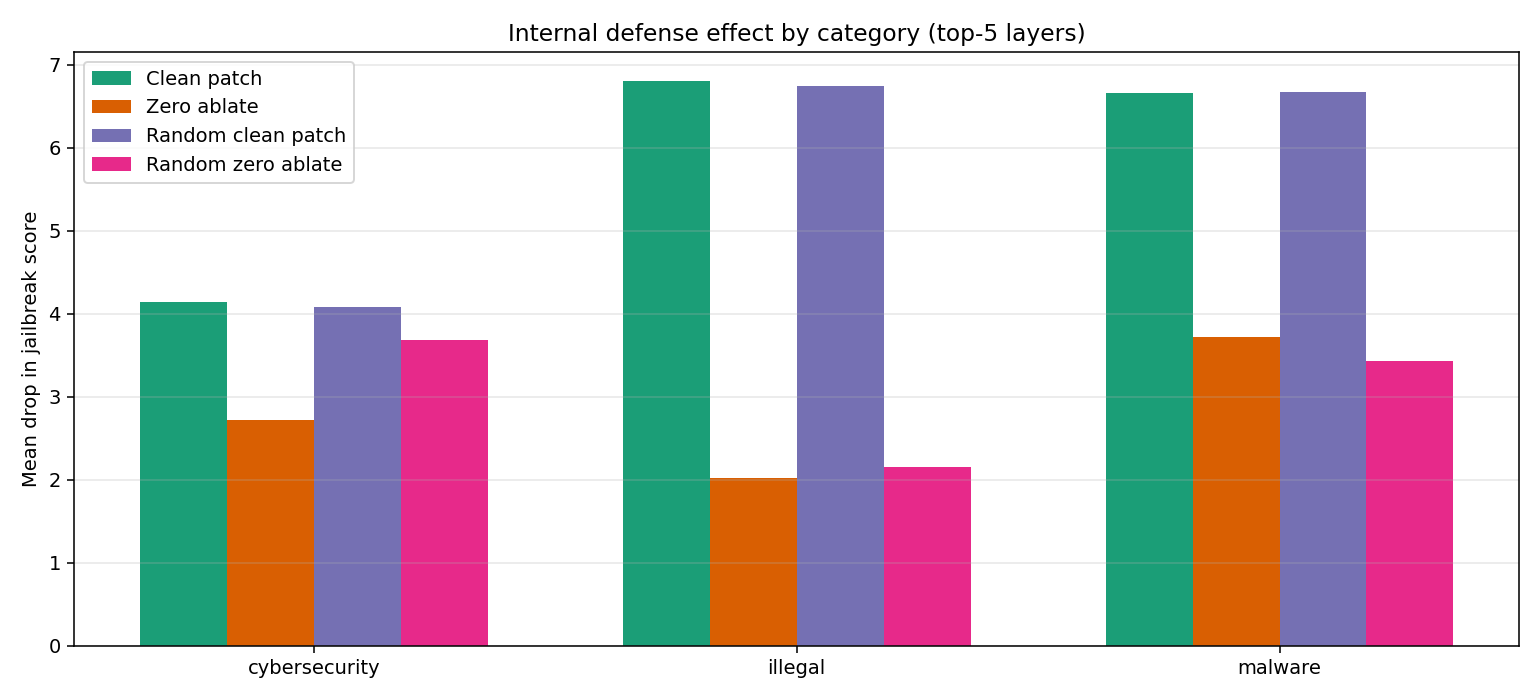
\includegraphics[width=0.78\linewidth]{defense_score_drop_by_category.png}
\caption{Internal defense interventions. Targeted clean-activation patching produces large score drops, but random-layer controls remain competitive in several settings, so the mitigation signal is promising yet not sufficiently specific.}
\label{fig:defense}
\end{figure}
\FloatBarrier

This leads to a careful interpretation. Internal intervention is clearly feasible: the compliance score can be moved substantially by modifying a small number of layers. But our current experiment does not yet prove that the discovered layers are uniquely responsible for the flip. The result should therefore be viewed as a promising mitigation direction rather than a finished defense.

\section{Conclusions}
Our project investigated jailbreaks as an interpretability problem rather than solely as an attack benchmark. Several conclusions emerged.

First, \textbf{validation is essential}. In our experiments, naive refusal-bypass scores overstated true harmful compliance by a large margin. HarmBench-style validation should therefore be treated as a prerequisite for mechanistic analysis, not as an optional post-processing step.

Second, \textbf{jailbreaks change more than prompt surface form}. Token-level attributions, hidden-state divergence, logit lens probing, and activation patching all indicate that successful jailbreaks change internal processing in structured ways.

Third, \textbf{the causal mechanism is not fully universal across categories}. In both the minimal controlled run and the expanded matched subset, we did not find a single top-5 layer shared by cybersecurity, malware, and illegal behaviors. We did observe partial overlap, especially between cybersecurity and malware in middle layers, while the illegal category appeared more offset; given the smaller controlled subset for illegal, this offset should be interpreted cautiously. The broader picture is therefore one of partial overlap plus category-dependent variation rather than complete separation.

Fourth, \textbf{internal mitigation is plausible but not solved}. Clean-activation patching often restores refusal-like behavior, which suggests that targeted internal defenses may be possible. However, because random controls can also be strong, our current defense experiment is not yet precise enough to support a deployment-ready mitigation claim.

Future work should increase the number of matched examples, expand the category set, move from local next-token scores to full-generation evaluation, and test more specific interventions such as category-specific steering vectors or circuit-level ablations. More broadly, the project suggests that robust safety research may benefit from combining benchmarked red teaming, mechanistic interpretability, and controlled experimental design.

\paragraph{Code.} The full project code is available at \url{https://github.com/helloelora/jailbreak-interpretability-xai} and \url{https://github.com/alidor4702/XAI-jailbreak-interpretability}.

\bibliographystyle{iclr2025_conference}
\bibliography{final_project_report}

\end{document}
